The measurement for this LIDAr was done by measuring the distance between  the sensor and an target, both rotating and while standstill (static) for to acquire the necessary data. Figure \ref{fig:testSetUp} describes how the test set up was done.
%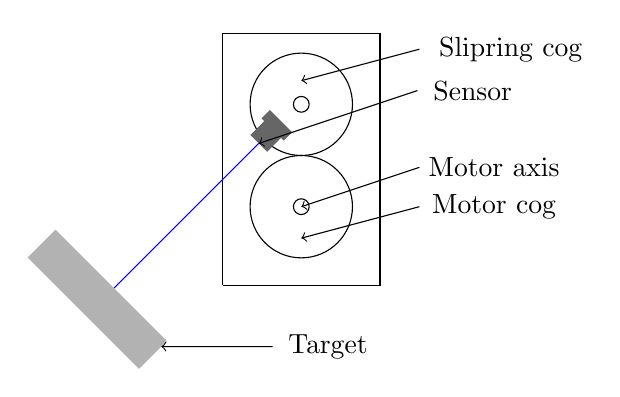
\begin{tikzpicture}[xscale=0.5, yscale=0.5]
\draw (0,0) -- (4,0) -- (4,6.4) -- (0,6.4) -- (0,0); %outre box
\draw (2,2) circle (1.3); %cog for motor
\draw (2,2) circle (0.2); % axis for motor
\draw (2,4.6) circle (1.3); %cog for slipring
\draw (2,4.6) circle (0.2); %axis for silp ring

%Sensor of the top cog
\fill[black!60!white, rotate=-45] (-2.3,4.0) rectangle (-1.5,3.7);
\fill[black!60!white, rotate=-45] (-2.2,3.2) rectangle (-1.6,3.8);
%beeam
\draw[blue, rotate=-45] (-1.9,3.2) -- (-1.9,-2);
%target
\fill[black!30!white, rotate=-45] (-4,-2) rectangle (0,-3);

%arrows
\draw[->, rotate=-45] (0,7)node[xshift=20] {Sensor} -- (-1.9,3.2);
\draw[->] (5,3)node[xshift=27] {Motor axis} -- (2.0,2.0) ;% motor axis
\draw[->] (5,2)node[xshift=27] {Motor cog} -- (2.0,1.2);% motor cog
\draw[->] (5,6)node[xshift=33] {Slipring cog} -- (2.0,5.2);% lidar cog
\draw[->, rotate=-45] (2,-0.2)node[xshift=20] {Target} -- (-0.0,-2.2);

\end{tikzpicture}
\begin{figure}[ht]
    \centering
   %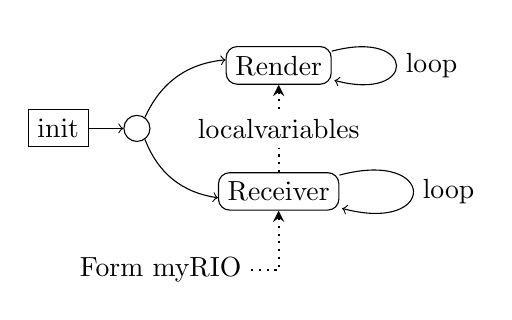
\begin{tikzpicture}
\tikzstyle{rounded} = [rectangle, rounded corners , minimum width=3mm, minimum height=1mm,text centered, draw=black]
\tikzstyle{round}=[circle, minimum width=0mm,draw=black]
\tikzstyle{square} = [rectangle, minimum width=1mm, draw=black]
\tikzstyle{empty}=[]

\usetikzlibrary{shapes.geometric, arrows}
\tikzstyle{arrow} = [thick,->,>=stealth]
\tikzstyle{dottarrow} = [thick, dotted,->,>=stealth]
\tikzstyle{dottline} = [thick, dotted,-,>=stealth]
\tikzstyle{noarrow}=[thick,-=,=stealth]

%nodes
\node (init) [square] {init};
\node (loop) [round, right of=init]{};
\node (render)[rounded, right of=loop, xshift=8mm, yshift=8mm ] {Render};
\node (rezive) [rounded, right of=loop, xshift=8mm, yshift=-8mm] {Receiver};
\node (datain) [empty, below of=rezive, xshift=-15mm]{Form myRIO};
\node (shared) [empty, below of=render, yshift=2mm]{localvariables};


%lines
%(Startnode)  edge [bend arrow]       node[text pos]  {text}          (target);
\path[->] 
(init) 		edge 								node[left]		{}			(loop)
(loop)		edge[bend left] 					node[left]		{}			(render)
(loop)		edge[bend right]					node[left]		{}			(rezive)
(render) 	edge[loop right]					node[right]		{loop}			(render)
(rezive) 	edge[loop right]					node[right]		{loop}			(rezive)
;
\draw [dottarrow] (datain) -| (rezive);
%\draw [dottarrow] (rezive) -- (render);
\draw [dottline] (rezive) -- (shared);
\draw [dottarrow] (shared) -- (render);

\end{tikzpicture}
   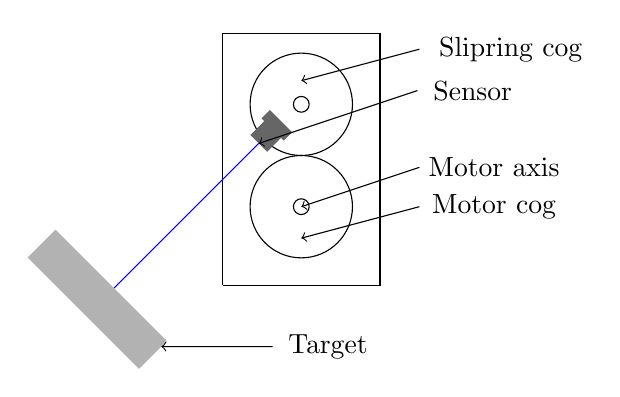
\begin{tikzpicture}[xscale=0.5, yscale=0.5]
\draw (0,0) -- (4,0) -- (4,6.4) -- (0,6.4) -- (0,0); %outre box
\draw (2,2) circle (1.3); %cog for motor
\draw (2,2) circle (0.2); % axis for motor
\draw (2,4.6) circle (1.3); %cog for slipring
\draw (2,4.6) circle (0.2); %axis for silp ring

%Sensor of the top cog
\fill[black!60!white, rotate=-45] (-2.3,4.0) rectangle (-1.5,3.7);
\fill[black!60!white, rotate=-45] (-2.2,3.2) rectangle (-1.6,3.8);
%beeam
\draw[blue, rotate=-45] (-1.9,3.2) -- (-1.9,-2);
%target
\fill[black!30!white, rotate=-45] (-4,-2) rectangle (0,-3);

%arrows
\draw[->, rotate=-45] (0,7)node[xshift=20] {Sensor} -- (-1.9,3.2);
\draw[->] (5,3)node[xshift=27] {Motor axis} -- (2.0,2.0) ;% motor axis
\draw[->] (5,2)node[xshift=27] {Motor cog} -- (2.0,1.2);% motor cog
\draw[->] (5,6)node[xshift=33] {Slipring cog} -- (2.0,5.2);% lidar cog
\draw[->, rotate=-45] (2,-0.2)node[xshift=20] {Target} -- (-0.0,-2.2);

\end{tikzpicture}
  \caption{The LIDAR had the construction with an slip ring to allow free passage of the cable without being twinned. Therefore it used 2 3D printed cogs to transfer the rotation from the motor to the sensor. The lower circle describe the cog that was connected to the motor whiles the top one with the sensor describe the cog that had an slip ring in it. There are also an target to the bottom left, how ever the distance is not up to scale hear for spacing reason.}
  \label{fig:testSetUp}
\end{figure}